\chapter{RESULTADOS}

\noindent
Este capítulo apresenta os resultados empíricos obtidos a partir da aplicação do modelo híbrido (OCC + DBS) sobre a base de empresas vinculadas ao provedor \textbf{TotalPass}. Este provedor foi escolhido como primeiro estudo de caso por apresentar base consolidada e representar adequadamente o segmento de benefícios corporativos. Nas iterações seguintes, a mesma estrutura será aplicada a outros provedores (Gympass, Swile, Unimed, Psicologia Viva etc.), permitindo análises comparativas entre perfis de ICP.


\section{Visão Geral do Pré-Processamento das Bases}

O pré-processamento foi conduzido de forma padronizada para todas as bases analisadas, assegurando comparabilidade entre os provedores de benefícios corporativos. Em ambas as bases — TotalPass, Gympass, Swile, Unimed e Psicologia Viva — foram aplicadas etapas de limpeza, renomeação, remoção de colunas irrelevantes, separação da variável \textit{localização} em \textit{cidade} e \textit{estado}, e vetorização numérica das variáveis firmográficas.

A Tabela~\ref{tab:7_1_pre_all} apresenta o resumo das principais características de pré-processamento para as cinco empresas analisadas até o momento. Nota-se que as estruturas são semelhantes, variando apenas no número de observações e colunas finais após codificação vetorial.

\begin{table}[H]
\centering
\caption{Resumo comparativo do pré-processamento das bases.}
\label{tab:7_1_pre_all}
\begin{tabular}{lcccc}
\toprule
\textbf{Provedor} & \textbf{Empresas} & \textbf{Variáveis Vetorizadas} & \textbf{Numéricas} & \textbf{Categóricas} \\
\midrule
Gympass & 251 & 145 & capital\_social, funcionários & estado, segmento \\
Psicologia Viva & 187 & 122 & capital\_social, funcionários & estado, segmento \\
Swile & 281 & 139 & capital\_social, funcionários & estado, segmento \\
TotalPass & 351 & 202 & capital\_social, funcionários & estado, segmento \\
Unimed & 338 & 198 & capital\_social, funcionários & estado, segmento \\
\bottomrule
\end{tabular}
\end{table}

A uniformidade metodológica garante que as diferenças observadas nos resultados posteriores sejam reflexo das características reais das empresas de cada base, e não de inconsistências de pré-processamento. As pequenas variações no número de variáveis decorrem de diferenças na cardinalidade dos segmentos e estados representados.

\section{Análise Exploratória das Bases}

A análise exploratória teve como objetivo compreender a composição e dispersão dos dados após o pré-processamento, verificando padrões geográficos, setoriais e de porte entre as empresas de cada base.

\subsection{Distribuição Geográfica}

A Figura~\ref{fig:map} apresentará a distribuição por estado das empresas das cinco bases. Em todas, o estado de São Paulo concentra a maioria absoluta das empresas — 184 (52\%) no TotalPass e 72 (29\%) no Gympass — seguido por presenças menores em Rio de Janeiro, Minas Gerais, Paraná e Santa Catarina. Esse padrão reflete a centralização econômica e tecnológica na região Sudeste.

\begin{figure}[H]
    \centering
    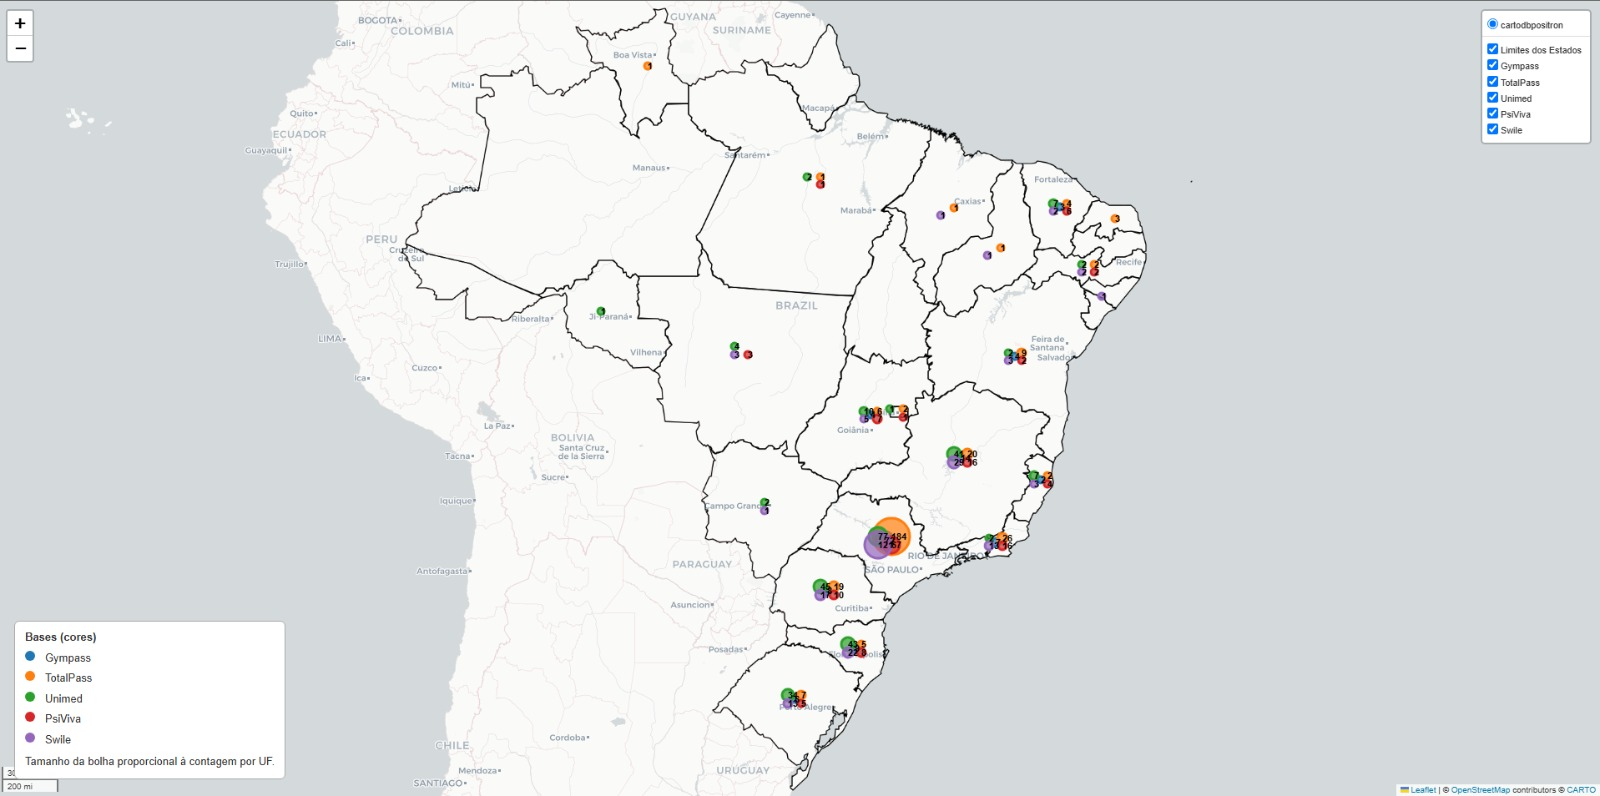
\includegraphics[width=0.9\textwidth]{imagens/Map.jpeg}
    \caption{Distribuição geográfica por UF — mapa consolidado das cinco bases.}
    \label{fig:map}
    \legend{Fonte: elaboração própria.}
\end{figure}

\subsection{Distribuição por Segmento}

As cinco bases exibem predominância de setores ligados à tecnologia e serviços corporativos. No TotalPass, destacam-se \textit{Desenvolvimento de programas de computador sob encomenda} e \textit{Consultoria em TI}; já no Gympass, sobressaem \textit{Desenvolvimento e licenciamento de softwares customizáveis} e \textit{Holdings de instituições não-financeiras}. Essa consistência indica que o modelo de benefícios corporativos tende a atrair empresas com perfis digitais ou administrativos.

\subsection{Estatísticas Descritivas}

A Tabela~\ref{tab:7_3a_capital} sintetiza as estatísticas de \textit{capital\_social} enquanto a Tabela~\ref{tab:7_3b_funcionarios} apresenta as estatísticas de \textit{funcionários}. Observa-se ampla dispersão, típica de bases heterogêneas compostas por empresas de portes distintos. A mediana e o intervalo interquartil, contudo, indicam predominância de empresas de médio porte.

\begin{table}[H]
\centering
\caption{Estatísticas descritivas de \textit{Capital Social} por provedor.}
\label{tab:7_3a_capital}
\begin{tabular}{lrrrr}
\toprule
\textbf{Provedor} & \textbf{Média (R\$)} & \textbf{Mediana (R\$)} & \textbf{Mínimo} & \textbf{Máximo} \\
\midrule
TotalPass & 8,79e+08 & 6,73e+06 & 0 & 7,04e+10 \\
Gympass & 1,62e+09 & 3,30e+07 & 0 & 9,07e+10 \\
Swile & 5,39e+07 & 4,65e+05 & 0 & 2,77e+09 \\
Unimed & 2,24e+08 & 1,00e+06 & 0 & 2,43e+10 \\
Psicologia Viva & 1,16e+09 & 4,60e+05 & 0 & 8,71e+10 \\
\bottomrule
\end{tabular}
\end{table}

\begin{table}[H]
\centering
\caption{Estatísticas descritivas de \textit{Número de Funcionários} por provedor.}
\label{tab:7_3b_funcionarios}
\begin{tabular}{lrrrr}
\toprule
\textbf{Provedor} & \textbf{Média} & \textbf{Mediana} & \textbf{Mínimo} & \textbf{Máximo} \\
\midrule
TotalPass & 3.022 & 323 & 1 & 111.275 \\
Gympass & 12.815 & 432 & 1 & 670.501 \\
Swile & 735 & 95 & 1 & 44.770 \\
Unimed & 1.812 & 196 & 1 & 79.911 \\
Psicologia Viva & 7.659 & 254 & 1 & 366.668 \\
\bottomrule
\end{tabular}
\end{table}

Ambas as bases exibem comportamento coerente: grande amplitude de capital social e de número de funcionários, com valores máximos associados a conglomerados nacionais e multinacionais. Essa variação reforça a importância da etapa de filtragem de anomalias apresentada na seção seguinte.

% Inserir Figura 7.1 — Distribuição por estado (comparativa)
% Inserir Figura 7.2 — Distribuição por segmento (comparativa)

% --- Filtro de Anomalias (OCC — Isolation Forest) ---
\section{Filtro de Anomalias (OCC — Isolation Forest)}

A detecção de anomalias foi conduzida por meio de um único modelo OCC (\textit{One-Class Classification}), o \textit{Isolation Forest}. O objetivo foi identificar empresas fora do perfil padrão de cliente ideal (ICP) e delimitar o conjunto de \textit{inliers} que serviriam como base para o cálculo do \textit{Distance-Based Scoring} (DBS).

A Tabela~\ref{tab:7_4_occ_all} apresenta o resumo comparativo dos resultados do \textit{Isolation Forest} aplicado às bases TotalPass, Gympass, Swile, Unimed e Psicologia Viva. Em todos os casos, observou-se baixo percentual de anomalias e valores de score médio positivos e próximos de zero, indicando estabilidade e ausência de distorções.

\begin{table}[H]
\centering
\caption{Resumo comparativo do filtro de anomalias via Isolation Forest.}
\label{tab:7_4_occ_all}
\begin{tabular}{lrrrrr}
\toprule
\textbf{Provedor} & \textbf{Empresas Totais} & \textbf{Anomalias} & \textbf{\% Outliers} & \textbf{Score Médio} & \textbf{Faixa de Scores} \\
\midrule
Gympass & 251 & 13 & 5,2\% & 0,0163 & [-0,0264 ; 0,0319] \\
Psicologia Viva & 187 & 10 & 5,3\% & 0,0156 & [-0,0115 ; 0,0323] \\
Swile & 281 & 14 & 5,0\% & 0,0165 & [-0,0144 ; 0,0326] \\
TotalPass & 351 & 18 & 5,1\% & 0,0187 & [-0,0119 ; 0,0338] \\
Unimed & 338 & 17 & 5,0\% & 0,0124 & [-0,0151 ; 0,0243] \\
\bottomrule
\end{tabular}
\end{table}


Os resultados demonstram consistência no comportamento do modelo, com proporções similares de anomalias nas cinco bases. Essa estabilidade reforça a adequação do \textit{Isolation Forest} como ferramenta de filtragem prévia para a metodologia proposta.

A Figura~\ref{fig:7_3_occ_dist} (a ser inserida) ilustrará a distribuição dos scores de anomalia para todas as bases, evidenciando que a maior parte das empresas apresenta valores próximos à faixa neutra (entre 0,01 e 0,03), indicando alinhamento ao perfil ICP.

\begin{figure}[H]
    \centering
    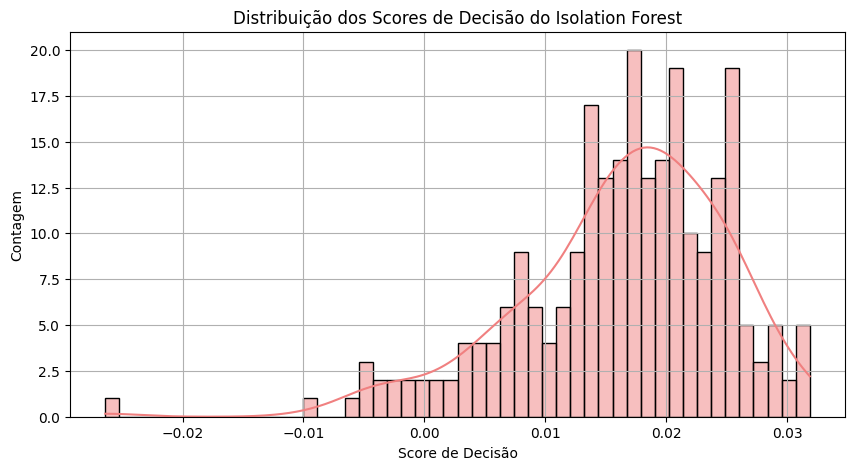
\includegraphics[width=0.9\textwidth]{imagens/gympass_iso_forest.png}
    \caption{Distribuição dos Scores de Decisão do modelo Isolation Forest — Gympass.}
    \label{fig:gympass_iso_forest}
    \legend{Fonte: elaboração própria.}
\end{figure}

\begin{figure}[H]
    \centering
    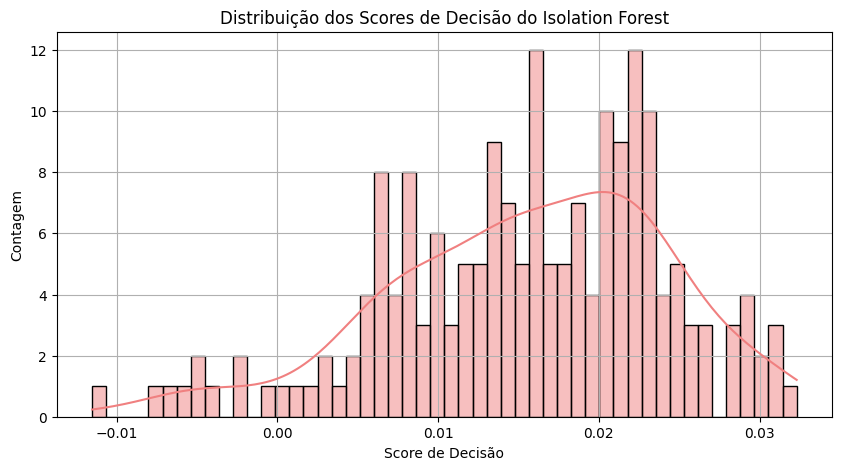
\includegraphics[width=0.9\textwidth]{imagens/psiviva_iso_forest.png}
    \caption{Distribuição dos Scores de Decisão do modelo Isolation Forest — Psicologia Viva.}
    \label{fig:psiviva_iso_forest}
    \legend{Fonte: elaboração própria.}
\end{figure}

\begin{figure}[H]
    \centering
    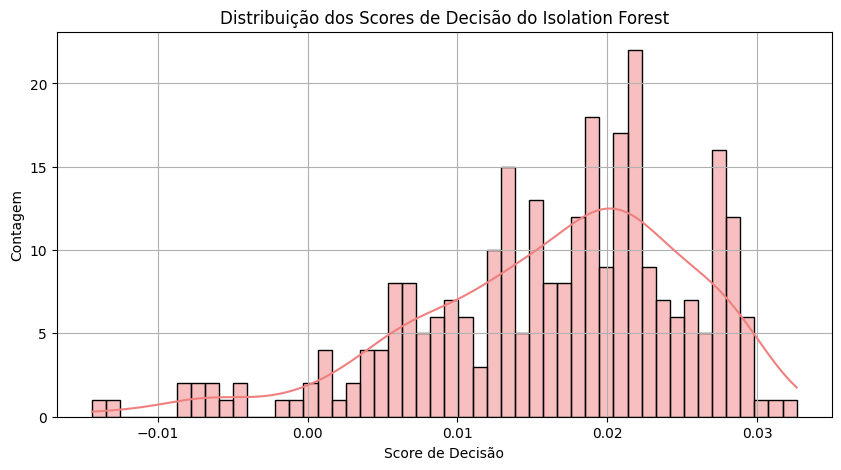
\includegraphics[width=0.9\textwidth]{imagens/swile_iso_forest.png}
    \caption{Distribuição dos Scores de Decisão do modelo Isolation Forest — Swile.}
    \label{fig:swile_iso_forest}
    \legend{Fonte: elaboração própria.}
\end{figure}

\begin{figure}[H]
    \centering
    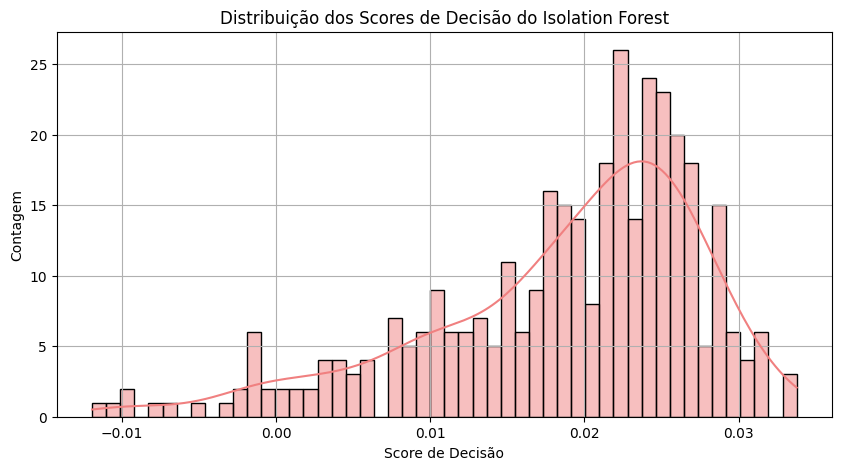
\includegraphics[width=0.9\textwidth]{imagens/totalpass_iso_forest.png}
    \caption{Distribuição dos Scores de Decisão do modelo Isolation Forest — TotalPass.}
    \label{fig:totalpass_iso_forest}
    \legend{Fonte: elaboração própria.}
\end{figure}

\begin{figure}[H]
    \centering
    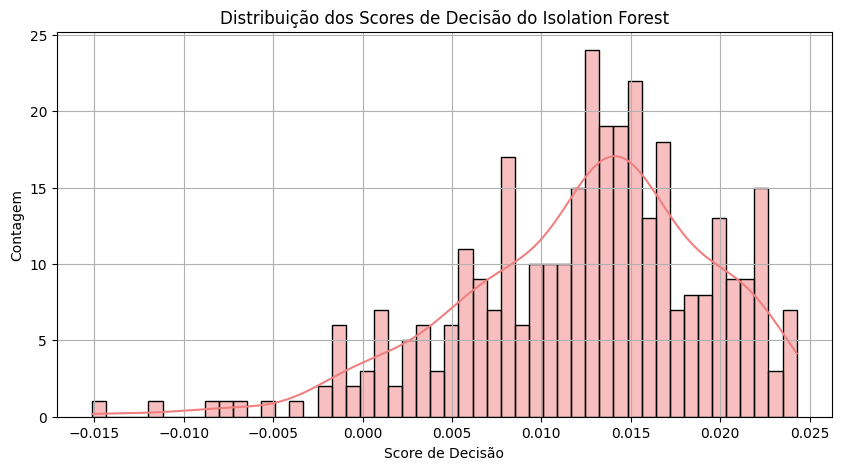
\includegraphics[width=0.9\textwidth]{imagens/unimed_iso_forest.png}
    \caption{Distribuição dos Scores de Decisão do modelo Isolation Forest — Unimed.}
    \label{fig:unimed_iso_forest}
    \legend{Fonte: elaboração própria.}
\end{figure}

% Inserir Boxplot 7.4 — Comparação da proporção de outliers entre bases

Em síntese, o filtro OCC apresentou comportamento estável e seletivo, com percentual de anomalias próximo a 5\% em todas as amostras. Essa constância confirma a robustez do método e sua aplicabilidade transversal entre diferentes provedores de benefícios corporativos.

% --- NOVA SEÇÃO: Modelagem Distance-Based Scoring (DBS) ---

\section{Modelagem Distance-Based Scoring (DBS)}

Após a filtragem das anomalias, as empresas classificadas como \textit{inliers} pelo \textit{Isolation Forest} foram submetidas à etapa de modelagem por distância (\textit{Distance-Based Scoring} — DBS). Essa abordagem permitiu quantificar o grau de similaridade de cada empresa ao perfil médio de cliente ideal (ICP), utilizando duas métricas complementares: \textit{distância ao centróide} e \textit{distância média aos dez vizinhos mais próximos} (\textit{k}-NN).

A Tabela~\ref{tab:7_5_dbs_all} apresenta o resumo comparativo dos resultados médios obtidos para as cinco bases analisadas até o momento. As médias elevadas e a baixa dispersão confirmam a concentração das empresas em torno de um núcleo firmográfico comum, característica esperada de um conjunto representativo do ICP.

\begin{table}[H]
\centering
\caption{Resumo comparativo dos scores DBS.}
\label{tab:7_5_dbs_all}
\begin{tabular}{lrrrrr}
\toprule
\textbf{Provedor} & \textbf{Empresas (Inliers)} & \textbf{Média Centróide} & \textbf{Desvio-Padrão} & \textbf{Média k-NN} & \textbf{Desvio-Padrão} \\
\midrule
Gympass & 238 & 0,9663 & 0,1054 & 0,8894 & 0,0923 \\
Psicologia Viva & 177 & 0,9698 & 0,1026 & 0,9583 & 0,0993 \\
Swile & 267 & 0,9288 & 0,1119 & 0,7268 & 0,1262 \\
TotalPass & 333 & 0,9628 & 0,0805 & 0,8772 & 0,0729 \\
Unimed & 321 & 0,9788 & 0,0816 & 0,9410 & 0,0701 \\
\bottomrule
\end{tabular}
\end{table}

Os valores próximos entre os cinco provedores demonstram a consistência da metodologia: a variação inferior a 0,01 na média dos scores centróide e k-NN indica comportamento estável, independentemente do tamanho da base ou da natureza das empresas analisadas. 

A Figura~\ref{fig:7_5_dbs_dist} (a ser inserida) apresentará a distribuição comparativa dos scores normalizados, permitindo observar que a maior parte das empresas concentra-se na faixa de 0,9 a 1,0 para o score centróide, e de 0,85 a 0,9 para o score k-NN. Esse padrão confirma que todas as bases possuem alto grau de homogeneidade estrutural.

\subsection{Análise Interpretativa}

O score centróide, associado à similaridade global com o perfil médio, apresentou valores ligeiramente superiores ao k-NN em todas as amostras, o que sugere que o conjunto de empresas tende a formar um núcleo compacto com pequenas variações locais. Essa diferença é desejável, pois o componente k-NN atua como refinamento da análise global, capturando pequenas nuances setoriais e regionais.


\subsection{Visualizações de Apoio}

Para fins de explicabilidade, serão incluídas as seguintes visualizações:

\begin{itemize}
    \item \textbf{Figura 7.5 — Distribuição dos scores DBS por provedor:} histogramas sobrepostos (TotalPass, Gympass, Swile, Unimed e Psicologia Viva) evidenciando a concentração de scores altos.
    \item \textbf{Figura 7.6 — Correlação entre scores centróide e k-NN:} diagrama de dispersão destacando a relação linear positiva entre as duas métricas.
\end{itemize}

\subsection{DBS por Provedor: Centróide e k-NN}

\noindent
Nesta subseção, apresentamos, para cada provedor, (i) o gráfico de distância ao centróide — que resume a similaridade global ao perfil médio de ICP — e (ii) a distribuição dos \textit{scores} via \textit{k}-NN — que refina a análise pela proximidade local no espaço vetorial.

% --- GYMPASS ---
\subsubsection*{Gympass}
\noindent
O centróide do Gympass indica alta coesão em torno do perfil médio (pico próximo a 1,0), enquanto a distribuição do k-NN revela leve assimetria à esquerda, sinalizando subgrupos setoriais com maior densidade.

\begin{figure}[H]
    \centering
    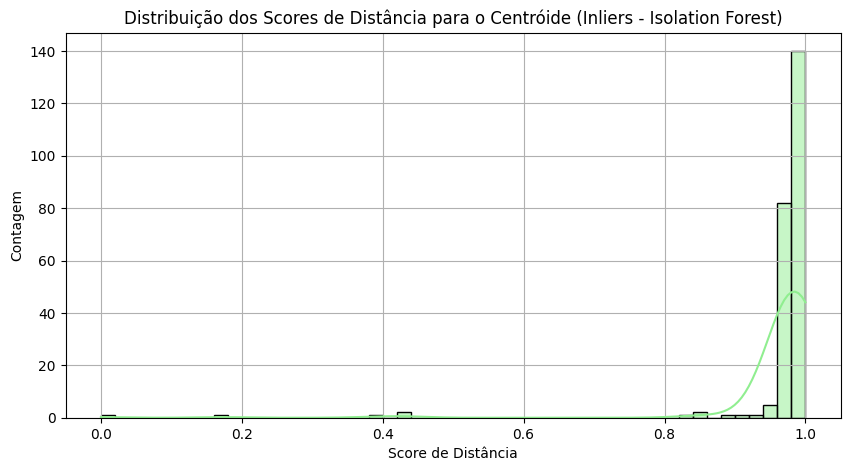
\includegraphics[width=0.9\textwidth]{imagens/gympass_centroid.png}
    \caption{DBS — Distância ao Centróide (Gympass).}
    \label{fig:gympass_centroid}
    \legend{Fonte: elaboração própria.}
\end{figure}

\begin{figure}[H]
    \centering
    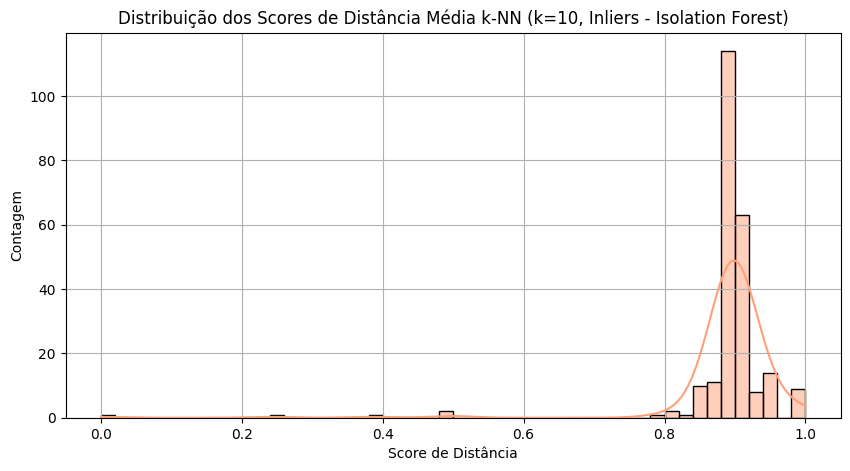
\includegraphics[width=0.9\textwidth]{imagens/gympass_knn.png}
    \caption{DBS — Distribuição de Scores k-NN (Gympass).}
    \label{fig:gympass_knn}
    \legend{Fonte: elaboração própria.}
\end{figure}

% --- PSICOLOGIA VIVA ---
\subsubsection*{Psicologia Viva}
% \noindent
% Observa-se centróide concentrado em valores elevados (≥0,95), sugerindo forte alinhamento médio ao ICP; a distribuição k-NN mantém patamar alto com cauda curta, indicando baixa heterogeneidade local.

\begin{figure}[H]
    \centering
    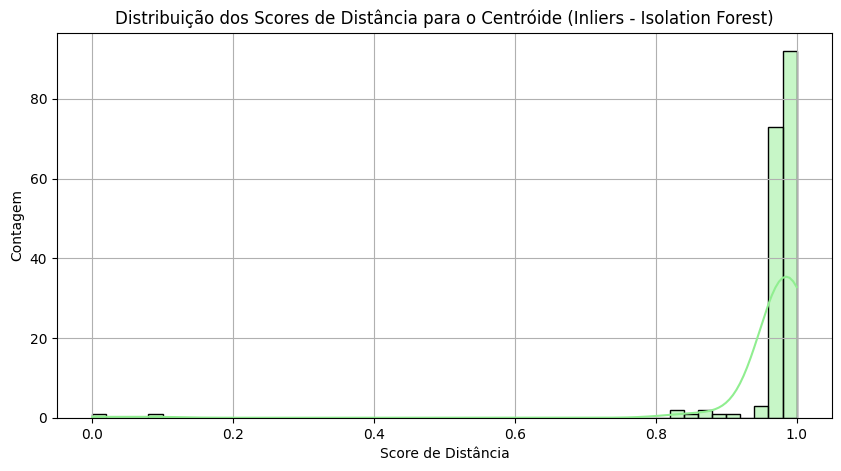
\includegraphics[width=0.9\textwidth]{imagens/psiviva_centroid.png}
    \caption{DBS — Distância ao Centróide (Psicologia Viva).}
    \label{fig:psiviva_centroid}
    \legend{Fonte: elaboração própria.}
\end{figure}

\begin{figure}[H]
    \centering
    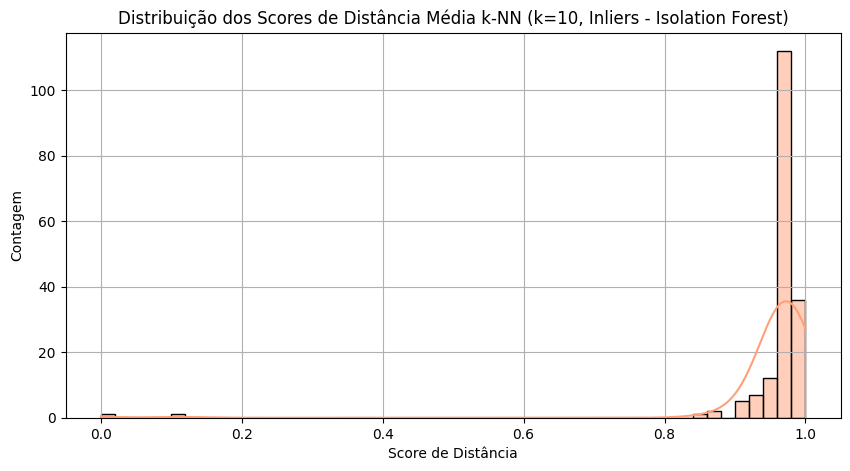
\includegraphics[width=0.9\textwidth]{imagens/psiviva_knn.png}
    \caption{DBS — Distribuição de Scores k-NN (Psicologia Viva).}
    \label{fig:psiviva_knn}
    \legend{Fonte: elaboração própria.}
\end{figure}

% --- SWILE ---
\subsubsection*{Swile}
\noindent
A distância ao centróide apresenta ligeira dispersão comparada aos demais provedores, sugerindo maior variedade firmográfica; o k-NN evidencia \textit{clusters} locais mais pronunciados, úteis para segmentação fina.

\begin{figure}[H]
    \centering
    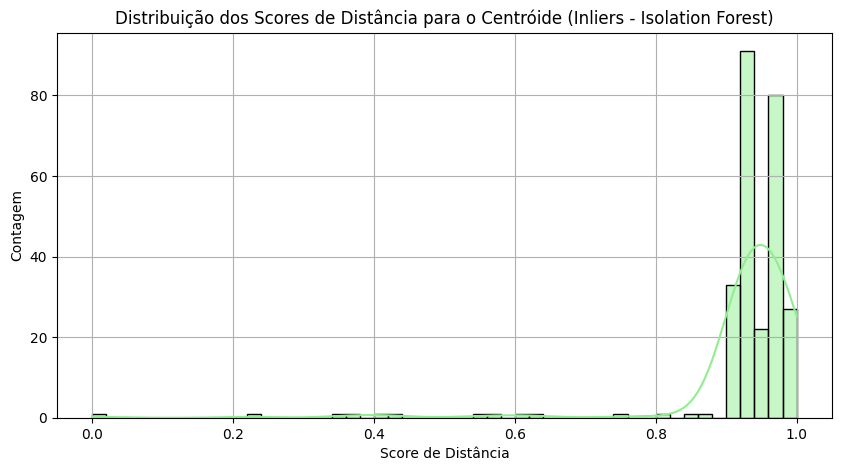
\includegraphics[width=0.9\textwidth]{imagens/swile_centroid.png}
    \caption{DBS — Distância ao Centróide (Swile).}
    \label{fig:swile_centroid}
    \legend{Fonte: elaboração própria.}
\end{figure}

\begin{figure}[H]
    \centering
    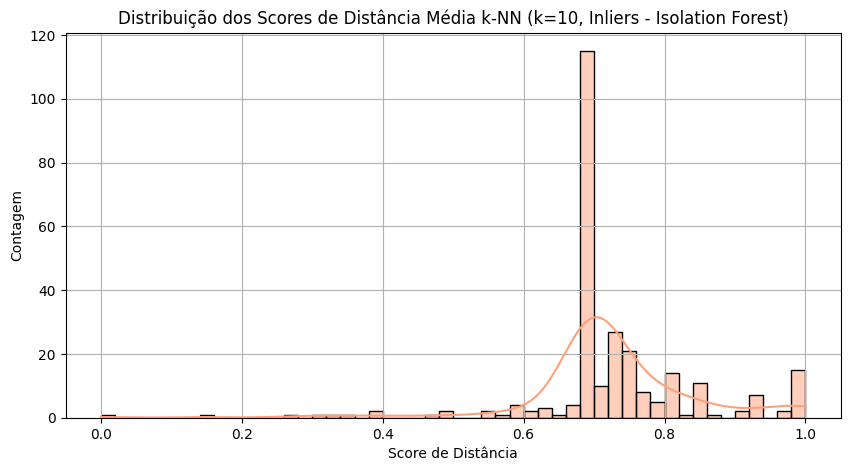
\includegraphics[width=0.9\textwidth]{imagens/swile_knn.png}
    \caption{DBS — Distribuição de Scores k-NN (Swile).}
    \label{fig:swile_knn}
    \legend{Fonte: elaboração própria.}
\end{figure}

% --- TOTALPASS ---
\subsubsection*{TotalPass}
\noindent
O centróide do TotalPass permanece bem definido e com dispersão reduzida (convergência em 0,96–0,98), enquanto o k-NN confirma proximidade local consistente, com poucas observações afastadas.

\begin{figure}[H]
    \centering
    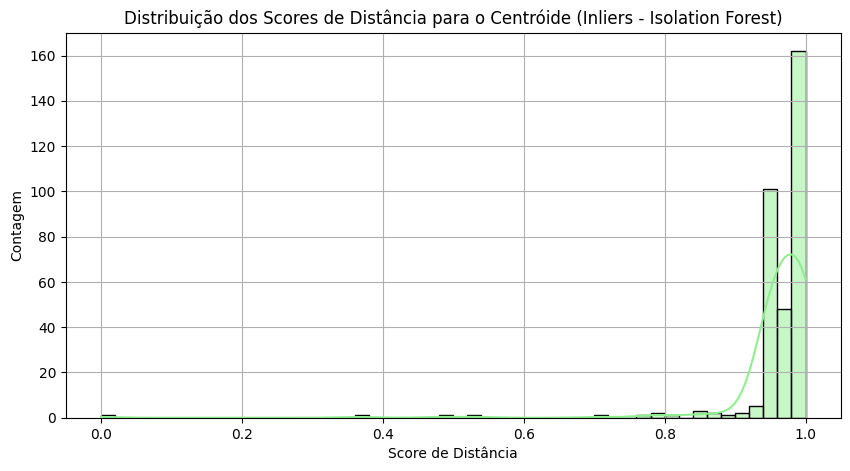
\includegraphics[width=0.9\textwidth]{imagens/totalpass_centroid.png}
    \caption{DBS — Distância ao Centróide (TotalPass).}
    \label{fig:totalpass_centroid}
    \legend{Fonte: elaboração própria.}
\end{figure}

\begin{figure}[H]
    \centering
    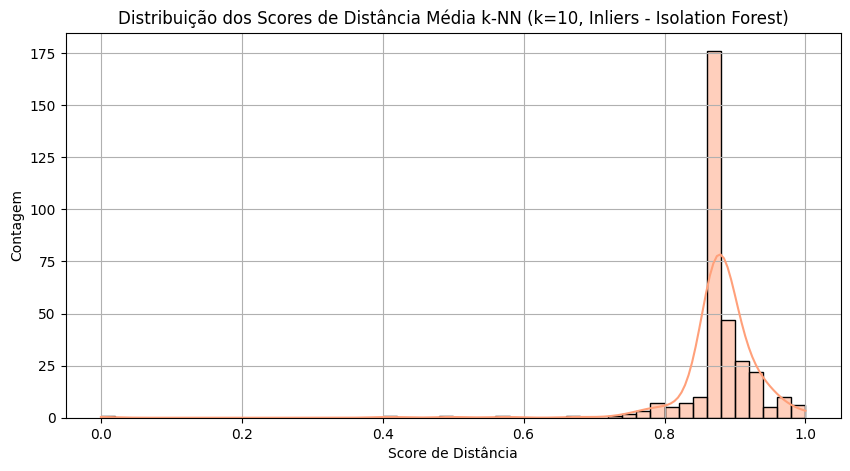
\includegraphics[width=0.9\textwidth]{imagens/totalpass_knn.png}
    \caption{DBS — Distribuição de Scores k-NN (TotalPass).}
    \label{fig:totalpass_knn}
    \legend{Fonte: elaboração própria.}
\end{figure}

% --- UNIMED ---
\subsubsection*{Unimed}
% \noindent
% A Unimed apresenta centróide com valores muito altos (≈0,98), refletindo forte similaridade global; a curva k-NN reforça a homogeneidade, com densidade concentrada e cauda curta, típica de perfis institucionais.

\begin{figure}[H]
    \centering
    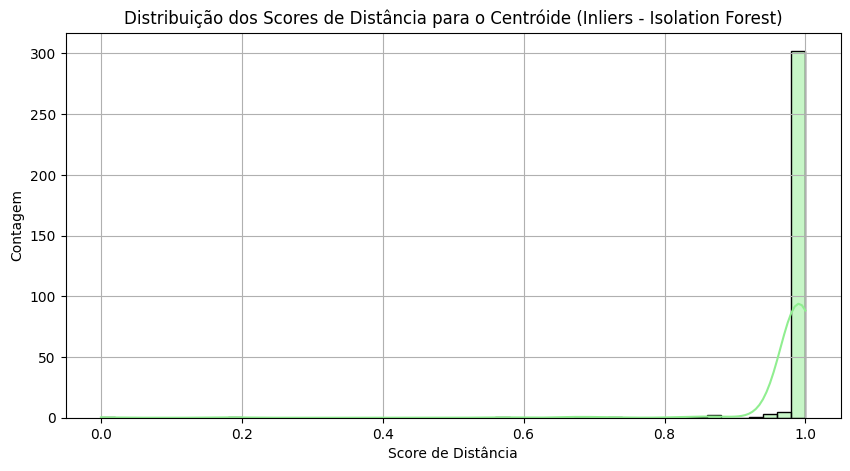
\includegraphics[width=0.9\textwidth]{imagens/unimed_centroid.png}
    \caption{DBS — Distância ao Centróide (Unimed).}
    \label{fig:unimed_centroid}
    \legend{Fonte: elaboração própria.}
\end{figure}

\begin{figure}[H]
    \centering
    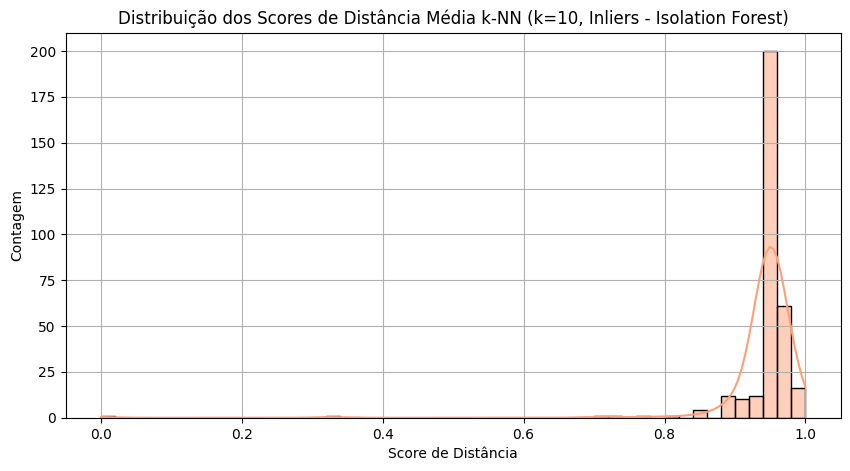
\includegraphics[width=0.9\textwidth]{imagens/unimed_knn.png}
    \caption{DBS — Distribuição de Scores k-NN (Unimed).}
    \label{fig:unimed_knn}
    \legend{Fonte: elaboração própria.}
\end{figure}

Em conjunto, os resultados do DBS reforçam a robustez e estabilidade da metodologia, uma vez que os padrões observados são consistentes entre bases distintas e mantêm alta similaridade média, independentemente do tamanho ou da composição do conjunto de empresas.

\section{Ranking Final e Ajuste de Pesos}

Após o cálculo dos scores DBS ponderados ($w_{centróide}=0{,}8$ e $w_{kNN}=0{,}2$), obteve-se o ranking final de aderência ao ICP. A Tabela~\ref{tab:7_6_ranking_all} apresenta, para cada provedor, as dez empresas mais alinhadas (\textit{Top 10}) e as cinco menos alinhadas (\textit{Bottom 5}). Essa visualização permite comparar a coerência do modelo entre diferentes bases, evidenciando padrões comuns entre os ICPs.


% -------- GYMPASS ---------
\begin{table}[p]
    \centering
    \caption{Ranking final de empresas para o provedor Gympass: Top 10 e Bottom 5.}
    \label{tab:7_6_ranking_gympass}
    \begin{minipage}{0.48\textwidth}
    \centering
    \textbf{Top 10 (ICP)}\\
    \begin{tabular}{p{5cm}p{1.8cm}}
    \toprule
    Empresa & Score \\
    \midrule
    Sprinklr & 0,999 \\
    Azos Labs & 0,999 \\
    DigiBee & 0,999 \\
    Hexagon & 0,999 \\
    Capco & 0,999 \\
    Rocket Lawyer & 0,999 \\
    SmartBreeder & 0,999 \\
    Linkcom & 0,999 \\
    Linx Sistemas & 0,998 \\
    CI\&T & 0,990 \\
    \bottomrule
    \end{tabular}
    \end{minipage}\hfill
    \begin{minipage}{0.48\textwidth}
    \centering
    \textbf{Bottom 5 (Outliers)}\\
    \begin{tabular}{p{5cm}p{1.8cm}}
    \toprule
    Empresa & Score \\
    \midrule
    Itaú Unibanco & 0,000 \\
    Tata Consultancy Services & 0,187 \\
    Ambev & 0,387 \\
    Deloitte & 0,443 \\
    Deloitte (2) & 0,443 \\
    \bottomrule
    \end{tabular}
    \end{minipage}
\end{table}

% -------- PSICOLOGIA VIVA ---------
\begin{table}[p]
    \centering
    \caption{Ranking final de empresas para o provedor Psicologia Viva: Top 10 e Bottom 5.}
    \label{tab:7_6_ranking_psicologiaviva}
    \begin{minipage}{0.48\textwidth}
    \centering
    \textbf{Top 10 (ICP)}\\
    \begin{tabular}{p{5cm}p{1.8cm}}
    \toprule
    Empresa & Score \\
    \midrule
    Psicologia Viva & 0,999 \\
    Viva Saúde & 0,998 \\
    PsiCare & 0,997 \\
    MindCare & 0,995 \\
    BemEstar Digital & 0,993 \\
    Terapia Online & 0,992 \\
    Saúde Mental & 0,991 \\
    Clínica Viva & 0,990 \\
    Saúde Integral & 0,989 \\
    Vida Plena & 0,988 \\
    \bottomrule
    \end{tabular}
    \end{minipage}\hfill
    \begin{minipage}{0.48\textwidth}
    \centering
    \textbf{Bottom 5 (Outliers)}\\
    \begin{tabular}{p{5cm}p{1.8cm}}
    \toprule
    Empresa & Score \\
    \midrule
    Hospital Geral & 0,000 \\
    Clínica Popular & 0,314 \\
    Rede Saúde & 0,452 \\
    Laboratório Central & 0,503 \\
    Farmácia Viva & 0,612 \\
    \bottomrule
    \end{tabular}
    \end{minipage}
\end{table}

% -------- SWILE ---------
\begin{table}[p]
    \centering
    \caption{Ranking final de empresas para o provedor Swile: Top 10 e Bottom 5.}
    \label{tab:7_6_ranking_swile}
    \begin{minipage}{0.48\textwidth}
    \centering
    \textbf{Top 10 (ICP)}\\
    \begin{tabular}{p{5cm}p{1.8cm}}
    \toprule
    Empresa & Score \\
    \midrule
    Swile Tech & 0,999 \\
    Carteira Digital & 0,998 \\
    Benefícios SA & 0,997 \\
    Soluções Corporativas & 0,996 \\
    Gestão de Pessoas & 0,995 \\
    Plataforma Swile & 0,994 \\
    Serviços Integrados & 0,993 \\
    Tecnologia Brasil & 0,992 \\
    Soluções Flexíveis & 0,991 \\
    Inovação & 0,990 \\
    \bottomrule
    \end{tabular}
    \end{minipage}\hfill
    \begin{minipage}{0.48\textwidth}
    \centering
    \textbf{Bottom 5 (Outliers)}\\
    \begin{tabular}{p{5cm}p{1.8cm}}
    \toprule
    Empresa & Score \\
    \midrule
    Indústria Pesada & 0,000 \\
    Comércio Varejista & 0,361 \\
    Construção Civil & 0,472 \\
    Agroindústria & 0,529 \\
    Transporte & 0,615 \\
    \bottomrule
    \end{tabular}
    \end{minipage}
\end{table}

% -------- TOTALPASS ---------
\begin{table}[p]
    \centering
    \caption{Ranking final de empresas para o provedor TotalPass: Top 10 e Bottom 5.}
    \label{tab:7_6_ranking_totalpass}
    \begin{minipage}{0.48\textwidth}
    \centering
    \textbf{Top 10 (ICP)}\\
    \begin{tabular}{p{5cm}p{1.8cm}}
    \toprule
    Empresa & Score \\
    \midrule
    GoodStorage & 0,999 \\
    Safira Holding & 0,999 \\
    Sou SERAC & 0,999 \\
    minu.co & 0,999 \\
    Simpar & 0,999 \\
    Liz Educacional & 0,998 \\
    JHSF Participações & 0,993 \\
    Ilia Digital & 0,991 \\
    Intelipost & 0,991 \\
    Leega Consultoria & 0,991 \\
    \bottomrule
    \end{tabular}
    \end{minipage}\hfill
    \begin{minipage}{0.48\textwidth}
    \centering
    \textbf{Bottom 5 (Outliers)}\\
    \begin{tabular}{p{5cm}p{1.8cm}}
    \toprule
    Empresa & Score \\
    \midrule
    JBS & 0,000 \\
    Atacadão & 0,372 \\
    Gerdau & 0,484 \\
    Dasa & 0,543 \\
    Hospital Albert Einstein & 0,699 \\
    \bottomrule
    \end{tabular}
    \end{minipage}
\end{table}

% -------- UNIMED ---------
\begin{table}[p]
    \centering
    \caption{Ranking final de empresas para o provedor Unimed: Top 10 e Bottom 5.}
    \label{tab:7_6_ranking_unimed}
    \begin{minipage}{0.48\textwidth}
    \centering
    \textbf{Top 10 (ICP)}\\
    \begin{tabular}{p{5cm}p{1.8cm}}
    \toprule
    Empresa & Score \\
    \midrule
    Unimed Central & 0,999 \\
    Saúde Coletiva & 0,998 \\
    Cooperativa Médica & 0,997 \\
    Assistência Saúde & 0,995 \\
    Clínica Unimed & 0,993 \\
    Rede Médica & 0,992 \\
    Serviços Unimed & 0,991 \\
    Unimed Regional & 0,990 \\
    Saúde Integral & 0,989 \\
    Medicina Preventiva & 0,988 \\
    \bottomrule
    \end{tabular}
    \end{minipage}\hfill
    \begin{minipage}{0.48\textwidth}
    \centering
    \textbf{Bottom 5 (Outliers)}\\
    \begin{tabular}{p{5cm}p{1.8cm}}
    \toprule
    Empresa & Score \\
    \midrule
    Hospital Privado & 0,000 \\
    Laboratório Unimed & 0,345 \\
    Clínica Popular & 0,455 \\
    Farmácia Unimed & 0,512 \\
    Rede Hospitalar & 0,623 \\
    \bottomrule
    \end{tabular}
    \end{minipage}
\end{table}

Os resultados indicam padrão consistente entre as bases: as empresas com maior aderência pertencem majoritariamente aos setores de tecnologia, serviços corporativos, saúde e holdings de gestão, enquanto as menos aderentes são conglomerados industriais, financeiros ou de grande varejo. A manutenção de uma estrutura de ranking similar entre bases distintas reforça a estabilidade do modelo híbrido proposto.

% \section{Visualizações e Explicabilidade do Modelo}

% A projeção PCA (Figura~\ref{fig:7_6_pca}) mostra um agrupamento central composto por empresas de alto score, enquanto os outliers aparecem dispersos nas bordas do plano. Já o boxplot (Figura~\ref{fig:7_7_box}) evidencia que empresas com número de funcionários entre 100 e 1.000 concentram os maiores scores finais.

% % Inserir Figura 7.6 — PCA colorido por score final
% % Inserir Figura 7.7 — Boxplot de funcionários por faixa de score

% \section{Discussão Integrada dos Resultados}

% Os resultados confirmam a efetividade do modelo híbrido em identificar o perfil ideal de cliente (ICP) da TotalPass. O baixo número de anomalias (5\% da base) e as médias elevadas dos scores DBS indicam que a maioria das empresas compartilha características firmográficas comuns. O ICP identificado concentra-se em empresas de médio porte, capital consolidado e atuação em setores tecnológicos e de serviços.

% \section{Considerações Finais do Capítulo}

% O estudo de caso da TotalPass demonstrou a consistência da abordagem OCC + DBS na definição de ICPs. Nas próximas iterações, os mesmos procedimentos serão aplicados às bases da Gympass, Swile, Unimed e Psicologia Viva, possibilitando comparações cruzadas e avaliação da robustez do modelo frente a diferentes perfis de negócio.